\documentclass[acmlarge]{acmart}

\usepackage{booktabs} % For formal tables


\usepackage[ruled]{algorithm2e} % For algorithms
\renewcommand{\algorithmcfname}{ALGORITHM}
\SetAlFnt{\small}
\SetAlCapFnt{\small}
\SetAlCapNameFnt{\small}
\SetAlCapHSkip{0pt}
\IncMargin{-\parindent}

% Metadata Information
%\acmJournal{PACMHCI}
%\acmVolume{9}
%\acmNumber{4}
%\acmArticle{39}
%\acmYear{2010}
%\acmMonth{3}
%\acmArticleSeq{11}


% DOI
\acmDOI{0000001.0000001}

% Paper history
%\received{February 2007}
%\received{March 2009}
%\received[accepted]{June 2009}


% Document starts
\begin{document}
% Title portion
\title{Security Suite: EECS 444 Final Project}
% \titlenote{We can add a note to the title}

\author{Kim Almcrantz}
\affiliation{\institution{Destroyer of Worlds}}
\email{kaa97@case.edu}

\author{Mark Lalor}
\affiliation{\institution{Eater of Nightmares}}
\email{mwl58@case.edu}

\author{Brian Li}
\affiliation{\institution{Summoner of Flames}}
\email{bvl8@case.edu}

\author{Vanessa Melikian}
\affiliation{\institution{Reaper of Souls}}
\email{vlm21@case.edu}

\author{Maya Nayak}
\affiliation{\institution{Tormentor of the Lost}}
\email{mkn30@case.edu}

\author{Jacob Wise}
\affiliation{\institution{Annihilator of the Innocent}}
\email{jsw107@case.edu}



\begin{abstract}
This is our abstract. Currently it is empty because no one has written it. In order to make it not empty, it must be written/
\end{abstract}

\keywords{encryption, cipher, hash, entropy}

\maketitle

% The default list of authors is too long for headers.
% \renewcommand{\shortauthors}{G. Zhou et al.}

\section{Introduction}\label{sec:intro}

To begin, we ponder a quote from an anonymous philosopher.
\begin{quote}
  ``where's brian ''.
\end{quote}
What does it mean? Who said it? Why was it said? We may never know. But what we do know is the following:

This article is divided into several sections, in Section [\ref{sec:intro}], we introduce the cryptographic environment that we will explore. In Section [\ref{sec:impl}] we describe implementations of several symmetric and asymmetric encryption algorithms, and then Section [\ref{sec:gui}] we present our tool \textsc{SecuritySuiteGUI}, a software suite to experiment with these implementations. We then demonstrate the power of password cracking with a hashcat demo in Section [\ref{sec:hashcat}]. Finally, we demonstrate how the Vigenère cipher may be easily cracked with computational power in Section [\ref{sec:vinegar}]. We evaluate our methods in Section [\ref{sec:evaluation}], and then discuss our techniques, challenges, and other thoughts in Section [\ref{sec:discussion}]. Finally, we discuss our final conclusions in Section [\ref{sec:conclusions}].

% itemize
\begin{itemize}
\item To the best of our knowledge, this is not the first time something like this was developed
\item We use \cite{Adya-01}, for a chocolate chip cookie recipe.
\end{itemize}

\subsection{Basic Crypto Stuff}

This is a talk about all the types of ciphers, symmetric, asymmetric, maybe more!

Here is the structure of the a bad algorithm:

\begin{enumerate}
\item Break into blocks of size $k=\frac{n^7}{8}$
\item Encipher each block with magic
\item Do XOR magic
\item Implement DES
\end{enumerate}

\section{Cryptographic Algorithm Implementations} \label{sec:impl}
\subsection{FakeDES}

As Algorithm~\ref{alg:one} states, DES is a symmetric encryption algorithm with steps.

% Algorithm
\begin{algorithm}[t]
\SetAlgoNoLine
\KwIn{Binary plaintext message $m$, a binary encryption key $k$}
\KwOut{Binary ciphertext message $c$}
$c$ = $m \times k$
\Repeat{$\pi > -1$}{
	$c = mc^2$
}
\caption{FakeDES implementation}
\label{alg:one}
\end{algorithm}

\subsection{RSA}

RSA is asymmetric!

\subsection{md5}

Md5 is a hash algorithm!

\section{SecuritySuiteGUI}\label{sec:gui}

% Figure
\begin{figure}
  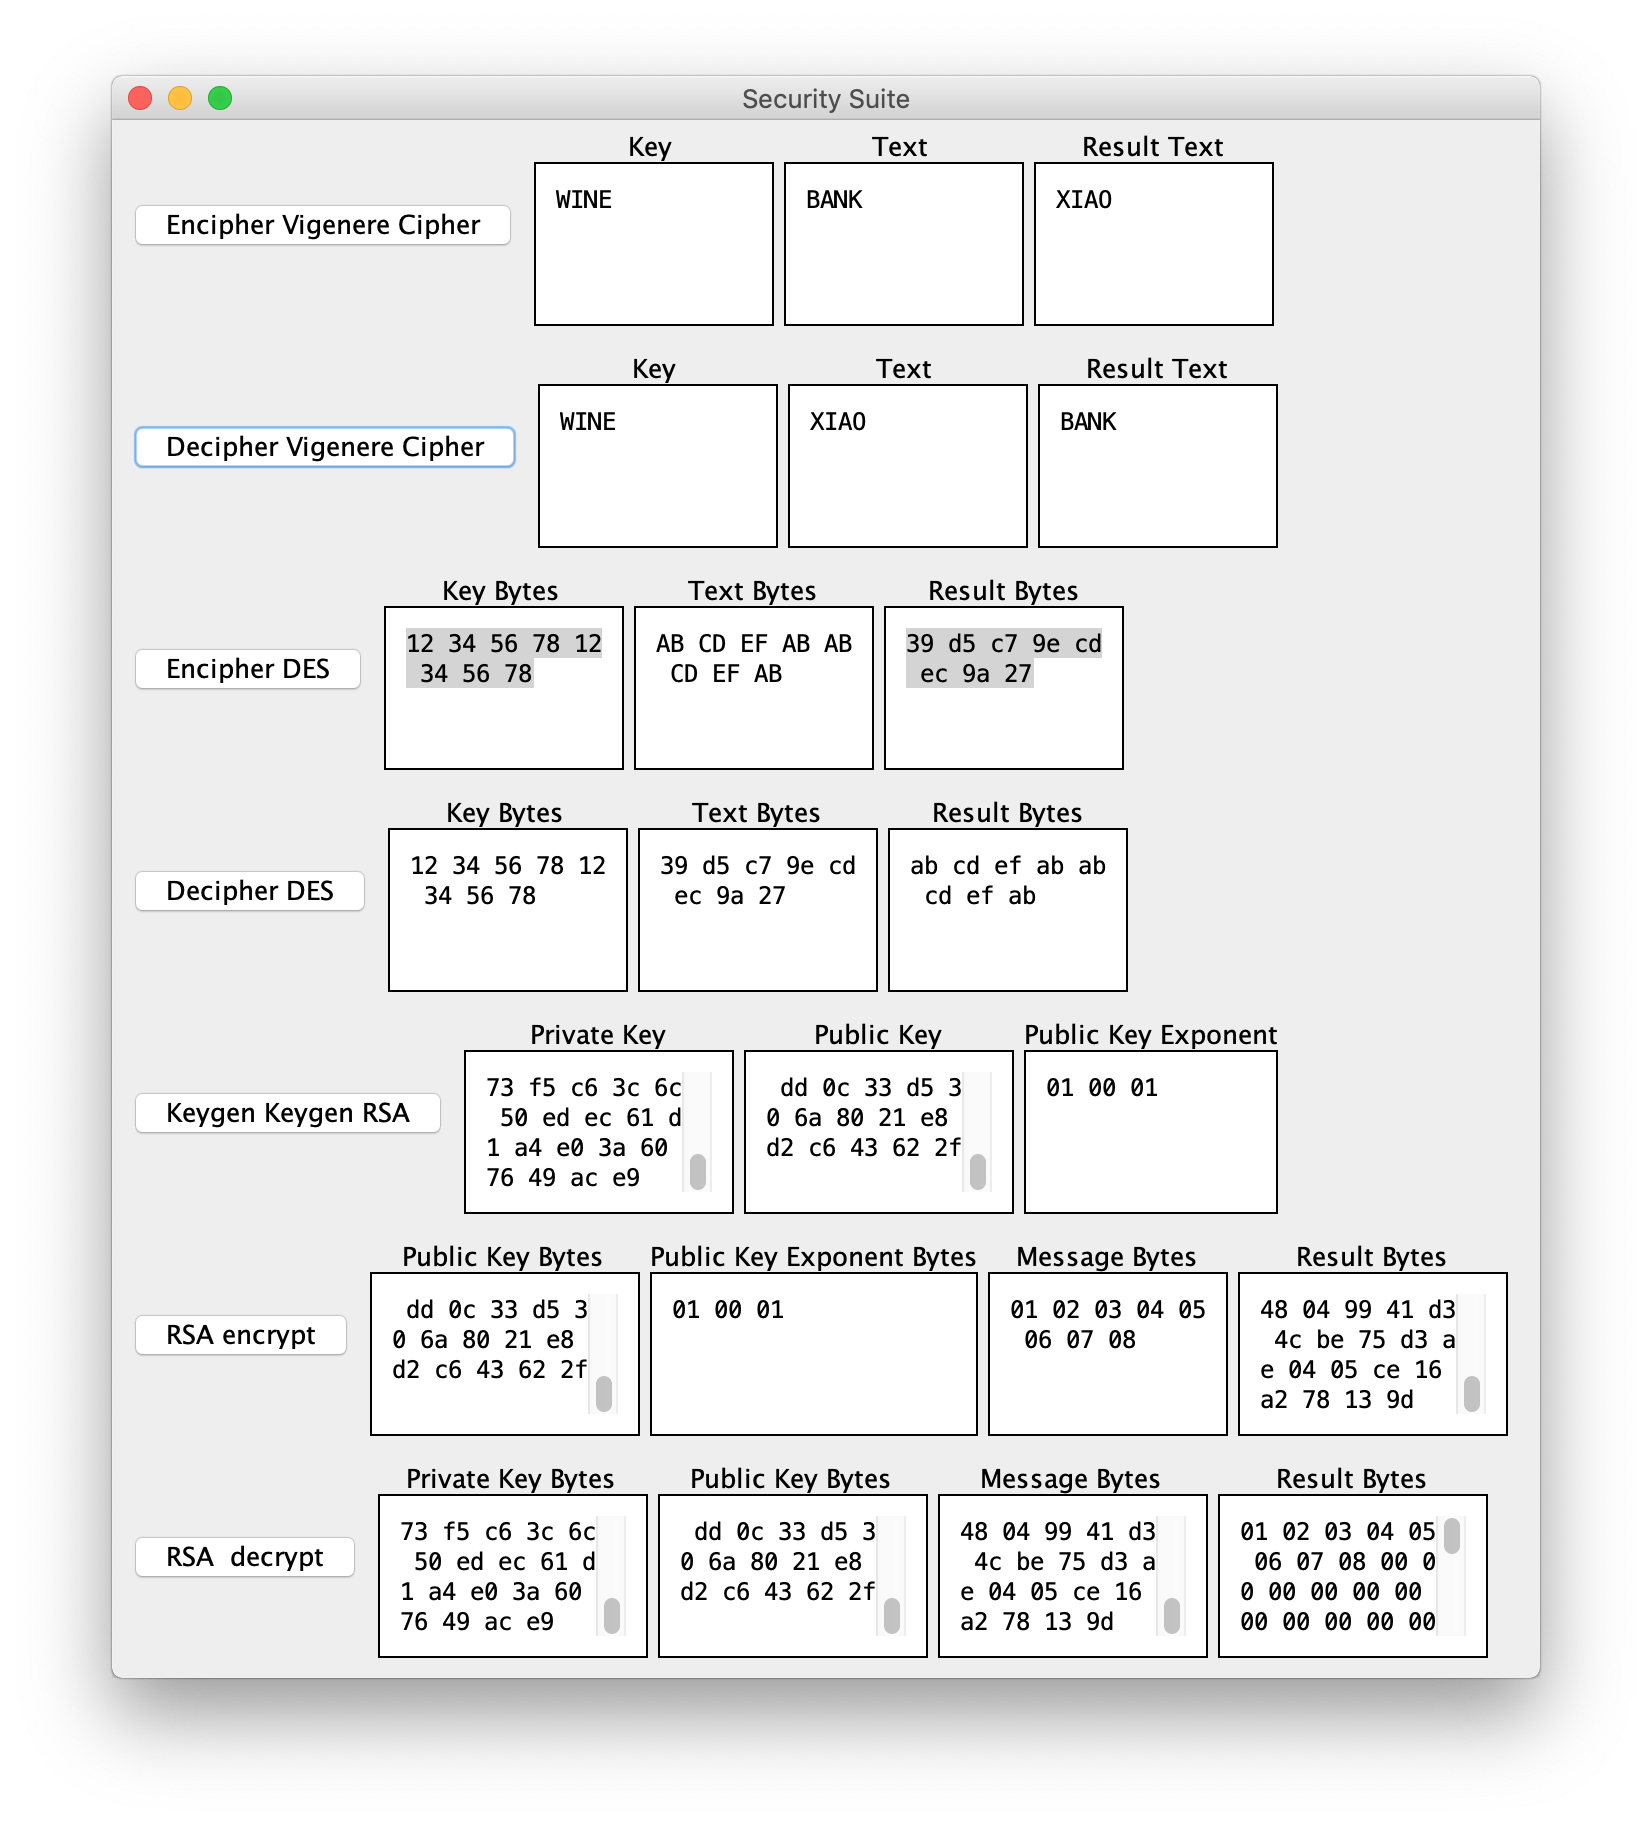
\includegraphics[scale=0.50]{demo}
  \Description{Image of our demo tool}
  \caption{Image of the security suite demo tool.}
  \label{fig:one}
\end{figure}

\subsection{Goals}

Some description:

\begin{lemma}[Lemma Subhead]The solution to the C-MWPC problem is no
worse than the solution to the MWPC.
\end{lemma}
\begin{proof}
Simply, any solution to the MWPC is also a solution to the
C-MWPC. But some solutions to C-MWPC may not apply to the MWPC (if any
coalescing were made).
\end{proof}

\section{Hashcat Demo}\label{sec:hashcat}

Words go here!

\section{Vigenère Cipher Cracker}\label{sec:vinegar}

Words go here too!

\section{Evaluation}\label{sec:evaluation}

Evaluation, efficiency? Challenges?

\section{Discussion}\label{sec:discussion}

What didn't we cover? :O

\section{Conclusions}\label{sec:conclusions}

We conclude that cryptography is very useful! $\frac{10}{10}$ would reccommend.

\section{References Samples}

A couple of citations with DOIs: \cite{2004:ITE:1009386.1010128, Kirschmer:2010:AEI:1958016.1958018}. Online citations: \cite{TUGInstmem, Thornburg01, CTANacmart}.

% Appendix
\appendix
\section{Elaboration on the ABCD algorithm}

This is an appendix, maybe about some equation
\begin{displaymath}
P=NP
\end{displaymath}

\section{Supplementary Materials}

\subsection{Hashcat materials}

Materials?

\subsection{Tool: Symmetric Ciphers Online }

\href{http://symmetric-ciphers.online-domain-tools.com/}{Link}

\begin{acks}

The authors would like to thank the mitochondria for being the powerhouse of the cell.

\end{acks}

% Bibliography
\bibliographystyle{ACM-Reference-Format}
\bibliography{sample-bibliography}

\end{document}
